\documentclass[twoside]{book}

% Packages required by doxygen
\usepackage{fixltx2e}
\usepackage{calc}
\usepackage{doxygen}
\usepackage[export]{adjustbox} % also loads graphicx
\usepackage{graphicx}
\usepackage[utf8]{inputenc}
\usepackage{makeidx}
\usepackage{multicol}
\usepackage{multirow}
\PassOptionsToPackage{warn}{textcomp}
\usepackage{textcomp}
\usepackage[nointegrals]{wasysym}
\usepackage[table]{xcolor}

% Font selection
\usepackage[T1]{fontenc}
\usepackage[scaled=.90]{helvet}
\usepackage{courier}
\usepackage{amssymb}
\usepackage{sectsty}
\renewcommand{\familydefault}{\sfdefault}
\allsectionsfont{%
  \fontseries{bc}\selectfont%
  \color{darkgray}%
}
\renewcommand{\DoxyLabelFont}{%
  \fontseries{bc}\selectfont%
  \color{darkgray}%
}
\newcommand{\+}{\discretionary{\mbox{\scriptsize$\hookleftarrow$}}{}{}}

% Page & text layout
\usepackage{geometry}
\geometry{%
  a4paper,%
  top=2.5cm,%
  bottom=2.5cm,%
  left=2.5cm,%
  right=2.5cm%
}
\tolerance=750
\hfuzz=15pt
\hbadness=750
\setlength{\emergencystretch}{15pt}
\setlength{\parindent}{0cm}
\setlength{\parskip}{3ex plus 2ex minus 2ex}
\makeatletter
\renewcommand{\paragraph}{%
  \@startsection{paragraph}{4}{0ex}{-1.0ex}{1.0ex}{%
    \normalfont\normalsize\bfseries\SS@parafont%
  }%
}
\renewcommand{\subparagraph}{%
  \@startsection{subparagraph}{5}{0ex}{-1.0ex}{1.0ex}{%
    \normalfont\normalsize\bfseries\SS@subparafont%
  }%
}
\makeatother

% Headers & footers
\usepackage{fancyhdr}
\pagestyle{fancyplain}
\fancyhead[LE]{\fancyplain{}{\bfseries\thepage}}
\fancyhead[CE]{\fancyplain{}{}}
\fancyhead[RE]{\fancyplain{}{\bfseries\leftmark}}
\fancyhead[LO]{\fancyplain{}{\bfseries\rightmark}}
\fancyhead[CO]{\fancyplain{}{}}
\fancyhead[RO]{\fancyplain{}{\bfseries\thepage}}
\fancyfoot[LE]{\fancyplain{}{}}
\fancyfoot[CE]{\fancyplain{}{}}
\fancyfoot[RE]{\fancyplain{}{\bfseries\scriptsize Generated by Doxygen }}
\fancyfoot[LO]{\fancyplain{}{\bfseries\scriptsize Generated by Doxygen }}
\fancyfoot[CO]{\fancyplain{}{}}
\fancyfoot[RO]{\fancyplain{}{}}
\renewcommand{\footrulewidth}{0.4pt}
\renewcommand{\chaptermark}[1]{%
  \markboth{#1}{}%
}
\renewcommand{\sectionmark}[1]{%
  \markright{\thesection\ #1}%
}

% Indices & bibliography
\usepackage{natbib}
\usepackage[titles]{tocloft}
\setcounter{tocdepth}{3}
\setcounter{secnumdepth}{5}
\makeindex

% Hyperlinks (required, but should be loaded last)
\usepackage{ifpdf}
\ifpdf
  \usepackage[pdftex,pagebackref=true]{hyperref}
\else
  \usepackage[ps2pdf,pagebackref=true]{hyperref}
\fi
\hypersetup{%
  colorlinks=true,%
  linkcolor=blue,%
  citecolor=blue,%
  unicode%
}

% Custom commands
\newcommand{\clearemptydoublepage}{%
  \newpage{\pagestyle{empty}\cleardoublepage}%
}

\usepackage{caption}
\captionsetup{labelsep=space,justification=centering,font={bf},singlelinecheck=off,skip=4pt,position=top}

%===== C O N T E N T S =====

\begin{document}

% Titlepage & ToC
\hypersetup{pageanchor=false,
             bookmarksnumbered=true,
             pdfencoding=unicode
            }
\pagenumbering{alph}
\begin{titlepage}
\vspace*{7cm}
\begin{center}%
{\Large Abstract Data Type List \\[1ex]\large 1.\+0 }\\
\vspace*{1cm}
{\large Generated by Doxygen 1.8.14}\\
\end{center}
\end{titlepage}
\clearemptydoublepage
\pagenumbering{roman}
\tableofcontents
\clearemptydoublepage
\pagenumbering{arabic}
\hypersetup{pageanchor=true}

%--- Begin generated contents ---
\chapter{List Abstract Data Type}
\label{md__r_e_a_d_m_e}
\Hypertarget{md__r_e_a_d_m_e}
An C++ Abstract Data Type implementation (Double Linked List)

\subsection*{Description}

A double linked list is a linked data structure that consists of a set of sequentially linked records called nodes. Each node contains three fields, that are references to the previous node, next node and the data that the node holds.

\subsection*{Compile}

Since the main goal on this project isn\textquotesingle{}t to create a main program, but instead, create a lib that can be used to create client\textquotesingle{}s codes, we will teach first how to include the lib inside your project.


\begin{DoxyEnumerate}
\item Download source code from this project, you can do it by cloning the git, downloading the zip, using wget...
\item Copy the source code ({\ttfamily \mbox{\hyperlink{list_8hpp_source}{list.\+hpp}}}) to your include folder inside your project.
\item Insert necessary {\ttfamily \#include}\textquotesingle{}s on your needed files
\item Compile the program and be happy about it!
\end{DoxyEnumerate}

\subsubsection*{Compile for this test}

In order to test the driver code, you can type inside de root folder of the project\+:


\begin{DoxyCode}
make
\end{DoxyCode}


and execute-\/it by calling\+:


\begin{DoxyCode}
./adt-list
\end{DoxyCode}


\section*{Authorship}

All codes here we\textquotesingle{}re made by Felipe Ramos for the E\+DB I course on U\+F\+RN. 
\chapter{Hierarchical Index}
\section{Class Hierarchy}
This inheritance list is sorted roughly, but not completely, alphabetically\+:\begin{DoxyCompactList}
\item \contentsline{section}{sc\+:\+:list$<$ T $>$\+:\+:const\+\_\+iterator}{\pageref{classsc_1_1list_1_1const__iterator}}{}
\begin{DoxyCompactList}
\item \contentsline{section}{sc\+:\+:list$<$ T $>$\+:\+:iterator}{\pageref{classsc_1_1list_1_1iterator}}{}
\end{DoxyCompactList}
\item \contentsline{section}{sc\+:\+:list$<$ T $>$}{\pageref{classsc_1_1list}}{}
\end{DoxyCompactList}

\chapter{Class Index}
\section{Class List}
Here are the classes, structs, unions and interfaces with brief descriptions\+:\begin{DoxyCompactList}
\item\contentsline{section}{\mbox{\hyperlink{classsc_1_1list_1_1const__iterator}{sc\+::list$<$ T $>$\+::const\+\_\+iterator}} \\*A simple \mbox{\hyperlink{classsc_1_1list_1_1const__iterator}{const\+\_\+iterator}} class }{\pageref{classsc_1_1list_1_1const__iterator}}{}
\item\contentsline{section}{\mbox{\hyperlink{classsc_1_1list_1_1iterator}{sc\+::list$<$ T $>$\+::iterator}} \\*A simple iterator class }{\pageref{classsc_1_1list_1_1iterator}}{}
\item\contentsline{section}{\mbox{\hyperlink{classsc_1_1list}{sc\+::list$<$ T $>$}} \\*Consists in the implementation of a double linked list using classes }{\pageref{classsc_1_1list}}{}
\end{DoxyCompactList}

\chapter{Class Documentation}
\hypertarget{classsc_1_1list_1_1const__iterator}{}\section{sc\+:\+:list$<$ T $>$\+:\+:const\+\_\+iterator Class Reference}
\label{classsc_1_1list_1_1const__iterator}\index{sc\+::list$<$ T $>$\+::const\+\_\+iterator@{sc\+::list$<$ T $>$\+::const\+\_\+iterator}}


A simple \mbox{\hyperlink{classsc_1_1list_1_1const__iterator}{const\+\_\+iterator}} class.  




{\ttfamily \#include $<$list.\+hpp$>$}

Inheritance diagram for sc\+:\+:list$<$ T $>$\+:\+:const\+\_\+iterator\+:\begin{figure}[H]
\begin{center}
\leavevmode
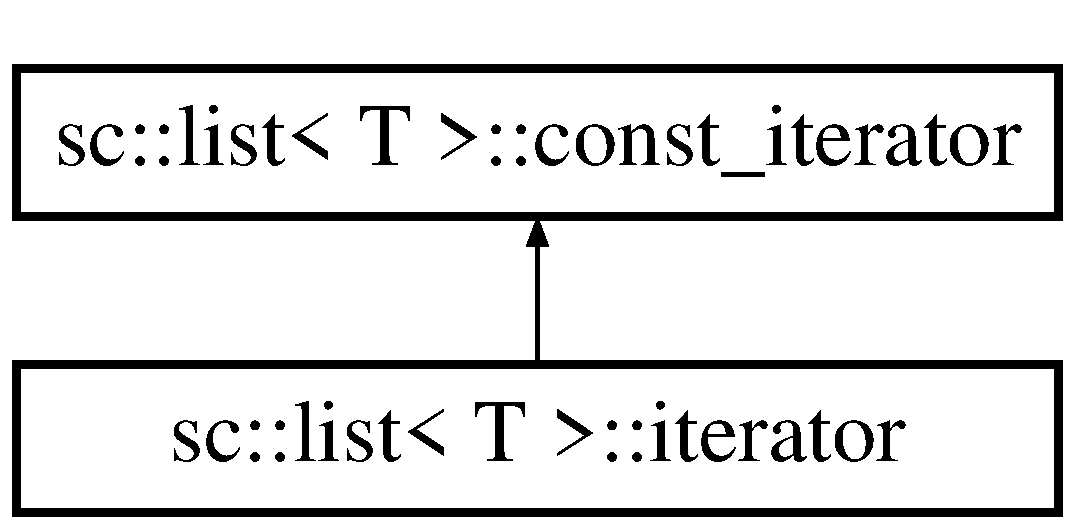
\includegraphics[height=2.000000cm]{classsc_1_1list_1_1const__iterator}
\end{center}
\end{figure}
\subsection*{Public Member Functions}
\begin{DoxyCompactItemize}
\item 
\mbox{\Hypertarget{classsc_1_1list_1_1const__iterator_a1df8ebba371776a05ee07ae91834ea92}\label{classsc_1_1list_1_1const__iterator_a1df8ebba371776a05ee07ae91834ea92}} 
\mbox{\hyperlink{classsc_1_1list_1_1const__iterator_a1df8ebba371776a05ee07ae91834ea92}{const\+\_\+iterator}} ()=default
\begin{DoxyCompactList}\small\item\em Default \mbox{\hyperlink{classsc_1_1list_1_1const__iterator}{const\+\_\+iterator}} initializer. \end{DoxyCompactList}\item 
\mbox{\Hypertarget{classsc_1_1list_1_1const__iterator_a32aafbcea528d2db2bc48a5bc81e46d8}\label{classsc_1_1list_1_1const__iterator_a32aafbcea528d2db2bc48a5bc81e46d8}} 
const T \& \mbox{\hyperlink{classsc_1_1list_1_1const__iterator_a32aafbcea528d2db2bc48a5bc81e46d8}{operator$\ast$}} () const
\begin{DoxyCompactList}\small\item\em Default \mbox{\hyperlink{classsc_1_1list_1_1const__iterator}{const\+\_\+iterator}} dereferencier. \end{DoxyCompactList}\item 
\mbox{\Hypertarget{classsc_1_1list_1_1const__iterator_a697f3bb58545ee5c3c0d8d821a2d6ccf}\label{classsc_1_1list_1_1const__iterator_a697f3bb58545ee5c3c0d8d821a2d6ccf}} 
\mbox{\hyperlink{classsc_1_1list_1_1const__iterator}{const\+\_\+iterator}} \& \mbox{\hyperlink{classsc_1_1list_1_1const__iterator_a697f3bb58545ee5c3c0d8d821a2d6ccf}{operator++}} ()
\begin{DoxyCompactList}\small\item\em Overload on the ++it operator. \end{DoxyCompactList}\item 
\mbox{\Hypertarget{classsc_1_1list_1_1const__iterator_aa563c3f71a41f9c3cc593013fa8b88c8}\label{classsc_1_1list_1_1const__iterator_aa563c3f71a41f9c3cc593013fa8b88c8}} 
\mbox{\hyperlink{classsc_1_1list_1_1const__iterator}{const\+\_\+iterator}} \mbox{\hyperlink{classsc_1_1list_1_1const__iterator_aa563c3f71a41f9c3cc593013fa8b88c8}{operator++}} (value\+\_\+type)
\begin{DoxyCompactList}\small\item\em Overload on the it++ operator. \end{DoxyCompactList}\item 
\mbox{\Hypertarget{classsc_1_1list_1_1const__iterator_aa400d21a07e6a88cd567754a323f06d8}\label{classsc_1_1list_1_1const__iterator_aa400d21a07e6a88cd567754a323f06d8}} 
\mbox{\hyperlink{classsc_1_1list_1_1const__iterator}{const\+\_\+iterator}} \& \mbox{\hyperlink{classsc_1_1list_1_1const__iterator_aa400d21a07e6a88cd567754a323f06d8}{operator-\/-\/}} ()
\begin{DoxyCompactList}\small\item\em Overload on the --it operator. \end{DoxyCompactList}\item 
\mbox{\Hypertarget{classsc_1_1list_1_1const__iterator_acfe2d659b4f43742714d057ea3a3d923}\label{classsc_1_1list_1_1const__iterator_acfe2d659b4f43742714d057ea3a3d923}} 
\mbox{\hyperlink{classsc_1_1list_1_1const__iterator}{const\+\_\+iterator}} \mbox{\hyperlink{classsc_1_1list_1_1const__iterator_acfe2d659b4f43742714d057ea3a3d923}{operator-\/-\/}} (value\+\_\+type)
\begin{DoxyCompactList}\small\item\em Overload on the it-- operator. \end{DoxyCompactList}\item 
\mbox{\Hypertarget{classsc_1_1list_1_1const__iterator_a6d27ecb7c15773b5f9f23b04107b112a}\label{classsc_1_1list_1_1const__iterator_a6d27ecb7c15773b5f9f23b04107b112a}} 
\mbox{\hyperlink{classsc_1_1list_1_1const__iterator}{const\+\_\+iterator}} \& \mbox{\hyperlink{classsc_1_1list_1_1const__iterator_a6d27ecb7c15773b5f9f23b04107b112a}{operator-\/}} (value\+\_\+type)
\begin{DoxyCompactList}\small\item\em Overload on the it -\/ value operator. \end{DoxyCompactList}\item 
\mbox{\Hypertarget{classsc_1_1list_1_1const__iterator_a18bdaa5189defdcd9b7f21587926263f}\label{classsc_1_1list_1_1const__iterator_a18bdaa5189defdcd9b7f21587926263f}} 
\mbox{\hyperlink{classsc_1_1list_1_1const__iterator}{const\+\_\+iterator}} \& \mbox{\hyperlink{classsc_1_1list_1_1const__iterator_a18bdaa5189defdcd9b7f21587926263f}{operator+}} (value\+\_\+type)
\begin{DoxyCompactList}\small\item\em Overload on the it + value operator. \end{DoxyCompactList}\item 
\mbox{\Hypertarget{classsc_1_1list_1_1const__iterator_a20f61345413f1ffe547c881e6bdc242f}\label{classsc_1_1list_1_1const__iterator_a20f61345413f1ffe547c881e6bdc242f}} 
bool \mbox{\hyperlink{classsc_1_1list_1_1const__iterator_a20f61345413f1ffe547c881e6bdc242f}{operator==}} (const \mbox{\hyperlink{classsc_1_1list_1_1const__iterator}{const\+\_\+iterator}} \&) const
\begin{DoxyCompactList}\small\item\em Overload on the == operator. \end{DoxyCompactList}\item 
\mbox{\Hypertarget{classsc_1_1list_1_1const__iterator_af23fb97b38945f60d4acdc9436f94efa}\label{classsc_1_1list_1_1const__iterator_af23fb97b38945f60d4acdc9436f94efa}} 
bool \mbox{\hyperlink{classsc_1_1list_1_1const__iterator_af23fb97b38945f60d4acdc9436f94efa}{operator!=}} (const \mbox{\hyperlink{classsc_1_1list_1_1const__iterator}{const\+\_\+iterator}} \&) const
\begin{DoxyCompactList}\small\item\em Overload on the != operator. \end{DoxyCompactList}\end{DoxyCompactItemize}
\subsection*{Protected Member Functions}
\begin{DoxyCompactItemize}
\item 
\mbox{\Hypertarget{classsc_1_1list_1_1const__iterator_abb42cbfb1699cb7427d9ab8a4d683b92}\label{classsc_1_1list_1_1const__iterator_abb42cbfb1699cb7427d9ab8a4d683b92}} 
\mbox{\hyperlink{classsc_1_1list_1_1const__iterator_abb42cbfb1699cb7427d9ab8a4d683b92}{const\+\_\+iterator}} (Node $\ast$p)
\begin{DoxyCompactList}\small\item\em Initialize the \mbox{\hyperlink{classsc_1_1list_1_1const__iterator}{const\+\_\+iterator}} to a Node. \end{DoxyCompactList}\end{DoxyCompactItemize}
\subsection*{Protected Attributes}
\begin{DoxyCompactItemize}
\item 
\mbox{\Hypertarget{classsc_1_1list_1_1const__iterator_ac8a1ecff3dcc804cd3fabfaf2360d461}\label{classsc_1_1list_1_1const__iterator_ac8a1ecff3dcc804cd3fabfaf2360d461}} 
Node $\ast$ \mbox{\hyperlink{classsc_1_1list_1_1const__iterator_ac8a1ecff3dcc804cd3fabfaf2360d461}{current}}
\begin{DoxyCompactList}\small\item\em Current Node that the iterator is on. \end{DoxyCompactList}\end{DoxyCompactItemize}
\subsection*{Friends}
\begin{DoxyCompactItemize}
\item 
\mbox{\Hypertarget{classsc_1_1list_1_1const__iterator_ab6cf03d50c50087700b0fb872accfa7b}\label{classsc_1_1list_1_1const__iterator_ab6cf03d50c50087700b0fb872accfa7b}} 
class \mbox{\hyperlink{classsc_1_1list_1_1const__iterator_ab6cf03d50c50087700b0fb872accfa7b}{list$<$ T $>$}}
\begin{DoxyCompactList}\small\item\em Get\textquotesingle{}s access to list$<$\+T$>$ methods. \end{DoxyCompactList}\end{DoxyCompactItemize}


\subsection{Detailed Description}
\subsubsection*{template$<$class T$>$\newline
class sc\+::list$<$ T $>$\+::const\+\_\+iterator}

A simple \mbox{\hyperlink{classsc_1_1list_1_1const__iterator}{const\+\_\+iterator}} class. 

The documentation for this class was generated from the following file\+:\begin{DoxyCompactItemize}
\item 
include/list.\+hpp\end{DoxyCompactItemize}

\hypertarget{classsc_1_1list_1_1iterator}{}\section{sc\+:\+:list$<$ T $>$\+:\+:iterator Class Reference}
\label{classsc_1_1list_1_1iterator}\index{sc\+::list$<$ T $>$\+::iterator@{sc\+::list$<$ T $>$\+::iterator}}


A simple iterator class.  




{\ttfamily \#include $<$list.\+hpp$>$}

Inheritance diagram for sc\+:\+:list$<$ T $>$\+:\+:iterator\+:\begin{figure}[H]
\begin{center}
\leavevmode
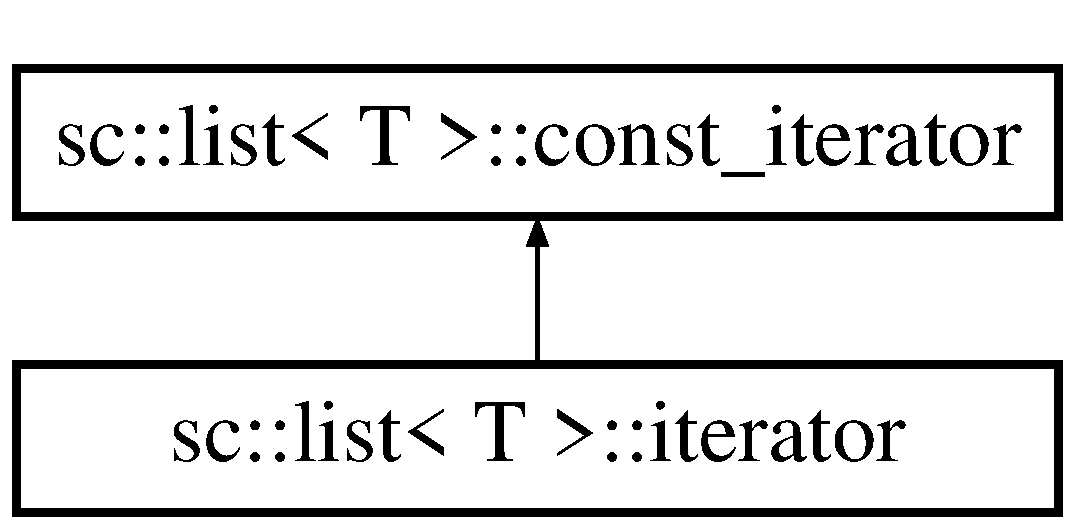
\includegraphics[height=2.000000cm]{classsc_1_1list_1_1iterator}
\end{center}
\end{figure}
\subsection*{Public Member Functions}
\begin{DoxyCompactItemize}
\item 
\mbox{\Hypertarget{classsc_1_1list_1_1iterator_acd90feec03d8a2762f36407a27166bb9}\label{classsc_1_1list_1_1iterator_acd90feec03d8a2762f36407a27166bb9}} 
\mbox{\hyperlink{classsc_1_1list_1_1iterator_acd90feec03d8a2762f36407a27166bb9}{iterator}} ()
\begin{DoxyCompactList}\small\item\em Default initializes the \mbox{\hyperlink{classsc_1_1list_1_1iterator_acd90feec03d8a2762f36407a27166bb9}{iterator()}} with \mbox{\hyperlink{classsc_1_1list_1_1const__iterator_a1df8ebba371776a05ee07ae91834ea92}{const\+\_\+iterator()}} methods. \end{DoxyCompactList}\item 
\mbox{\Hypertarget{classsc_1_1list_1_1iterator_a8e1feb979567a3fa27add54563d0008f}\label{classsc_1_1list_1_1iterator_a8e1feb979567a3fa27add54563d0008f}} 
const T \& \mbox{\hyperlink{classsc_1_1list_1_1iterator_a8e1feb979567a3fa27add54563d0008f}{operator$\ast$}} () const
\begin{DoxyCompactList}\small\item\em Default desreferencier of the iterator class. \end{DoxyCompactList}\item 
\mbox{\Hypertarget{classsc_1_1list_1_1iterator_aed5c46c8e0c470a9eccb5e47d0c80f4c}\label{classsc_1_1list_1_1iterator_aed5c46c8e0c470a9eccb5e47d0c80f4c}} 
\mbox{\hyperlink{classsc_1_1list_1_1iterator}{iterator}} \& \mbox{\hyperlink{classsc_1_1list_1_1iterator_aed5c46c8e0c470a9eccb5e47d0c80f4c}{operator++}} ()
\begin{DoxyCompactList}\small\item\em Overload on the ++it operator. \end{DoxyCompactList}\item 
\mbox{\Hypertarget{classsc_1_1list_1_1iterator_af3fb0443a14cecf4c2fc4e43a2701c51}\label{classsc_1_1list_1_1iterator_af3fb0443a14cecf4c2fc4e43a2701c51}} 
\mbox{\hyperlink{classsc_1_1list_1_1iterator}{iterator}} \mbox{\hyperlink{classsc_1_1list_1_1iterator_af3fb0443a14cecf4c2fc4e43a2701c51}{operator++}} (value\+\_\+type)
\begin{DoxyCompactList}\small\item\em Overload on the it++ operator. \end{DoxyCompactList}\item 
\mbox{\Hypertarget{classsc_1_1list_1_1iterator_abf189d629eae1b86654039bc923f3979}\label{classsc_1_1list_1_1iterator_abf189d629eae1b86654039bc923f3979}} 
\mbox{\hyperlink{classsc_1_1list_1_1iterator}{iterator}} \& \mbox{\hyperlink{classsc_1_1list_1_1iterator_abf189d629eae1b86654039bc923f3979}{operator-\/-\/}} ()
\begin{DoxyCompactList}\small\item\em Overload on the --it operator. \end{DoxyCompactList}\item 
\mbox{\Hypertarget{classsc_1_1list_1_1iterator_ac88b0479a79f2638b787d2f78cc50038}\label{classsc_1_1list_1_1iterator_ac88b0479a79f2638b787d2f78cc50038}} 
\mbox{\hyperlink{classsc_1_1list_1_1iterator}{iterator}} \mbox{\hyperlink{classsc_1_1list_1_1iterator_ac88b0479a79f2638b787d2f78cc50038}{operator-\/-\/}} (value\+\_\+type)
\begin{DoxyCompactList}\small\item\em Overload on the it-- operator. \end{DoxyCompactList}\item 
\mbox{\Hypertarget{classsc_1_1list_1_1iterator_adb805d53d2f2543d0b8b1cff44505e47}\label{classsc_1_1list_1_1iterator_adb805d53d2f2543d0b8b1cff44505e47}} 
\mbox{\hyperlink{classsc_1_1list_1_1iterator}{iterator}} \& \mbox{\hyperlink{classsc_1_1list_1_1iterator_adb805d53d2f2543d0b8b1cff44505e47}{operator-\/}} (value\+\_\+type)
\begin{DoxyCompactList}\small\item\em Overload on the it -\/ value operator. \end{DoxyCompactList}\item 
\mbox{\Hypertarget{classsc_1_1list_1_1iterator_a4aac68c89d98489a6fa94a9e13dcb1fc}\label{classsc_1_1list_1_1iterator_a4aac68c89d98489a6fa94a9e13dcb1fc}} 
\mbox{\hyperlink{classsc_1_1list_1_1iterator}{iterator}} \& \mbox{\hyperlink{classsc_1_1list_1_1iterator_a4aac68c89d98489a6fa94a9e13dcb1fc}{operator+}} (value\+\_\+type)
\begin{DoxyCompactList}\small\item\em Overload on the it + value operator. \end{DoxyCompactList}\item 
\mbox{\Hypertarget{classsc_1_1list_1_1iterator_a2cf562f77662ada512405bc6316f63f5}\label{classsc_1_1list_1_1iterator_a2cf562f77662ada512405bc6316f63f5}} 
bool \mbox{\hyperlink{classsc_1_1list_1_1iterator_a2cf562f77662ada512405bc6316f63f5}{operator==}} (const \mbox{\hyperlink{classsc_1_1list_1_1iterator}{iterator}} \&) const
\begin{DoxyCompactList}\small\item\em Overload on the == operator. \end{DoxyCompactList}\item 
\mbox{\Hypertarget{classsc_1_1list_1_1iterator_a029b713787de6e1402aae2079bba9f95}\label{classsc_1_1list_1_1iterator_a029b713787de6e1402aae2079bba9f95}} 
bool \mbox{\hyperlink{classsc_1_1list_1_1iterator_a029b713787de6e1402aae2079bba9f95}{operator!=}} (const \mbox{\hyperlink{classsc_1_1list_1_1iterator}{iterator}} \&) const
\begin{DoxyCompactList}\small\item\em Overload on the != operator. \end{DoxyCompactList}\end{DoxyCompactItemize}
\subsection*{Protected Member Functions}
\begin{DoxyCompactItemize}
\item 
\mbox{\Hypertarget{classsc_1_1list_1_1iterator_a818795d7651516a93e563f3229e86351}\label{classsc_1_1list_1_1iterator_a818795d7651516a93e563f3229e86351}} 
\mbox{\hyperlink{classsc_1_1list_1_1iterator_a818795d7651516a93e563f3229e86351}{iterator}} (Node $\ast$p)
\begin{DoxyCompactList}\small\item\em Default initializes the iterator with a node. \end{DoxyCompactList}\end{DoxyCompactItemize}
\subsection*{Friends}
\begin{DoxyCompactItemize}
\item 
\mbox{\Hypertarget{classsc_1_1list_1_1iterator_ab6cf03d50c50087700b0fb872accfa7b}\label{classsc_1_1list_1_1iterator_ab6cf03d50c50087700b0fb872accfa7b}} 
class \mbox{\hyperlink{classsc_1_1list_1_1iterator_ab6cf03d50c50087700b0fb872accfa7b}{list$<$ T $>$}}
\begin{DoxyCompactList}\small\item\em Get\textquotesingle{}s access to all list$<$\+T$>$ methods. \end{DoxyCompactList}\end{DoxyCompactItemize}
\subsection*{Additional Inherited Members}


\subsection{Detailed Description}
\subsubsection*{template$<$class T$>$\newline
class sc\+::list$<$ T $>$\+::iterator}

A simple iterator class. 

The documentation for this class was generated from the following file\+:\begin{DoxyCompactItemize}
\item 
include/list.\+hpp\end{DoxyCompactItemize}

\hypertarget{classsc_1_1list}{}\section{sc\+:\+:list$<$ T $>$ Class Template Reference}
\label{classsc_1_1list}\index{sc\+::list$<$ T $>$@{sc\+::list$<$ T $>$}}


Consists in the implementation of a double linked list using classes.  




{\ttfamily \#include $<$list.\+hpp$>$}

\subsection*{Classes}
\begin{DoxyCompactItemize}
\item 
class \mbox{\hyperlink{classsc_1_1list_1_1const__iterator}{const\+\_\+iterator}}
\begin{DoxyCompactList}\small\item\em A simple \mbox{\hyperlink{classsc_1_1list_1_1const__iterator}{const\+\_\+iterator}} class. \end{DoxyCompactList}\item 
class \mbox{\hyperlink{classsc_1_1list_1_1iterator}{iterator}}
\begin{DoxyCompactList}\small\item\em A simple iterator class. \end{DoxyCompactList}\end{DoxyCompactItemize}
\subsection*{Public Member Functions}
\begin{DoxyCompactItemize}
\item 
\mbox{\Hypertarget{classsc_1_1list_ab78427459eb9bc9886b6a581a2c9c216}\label{classsc_1_1list_ab78427459eb9bc9886b6a581a2c9c216}} 
\mbox{\hyperlink{classsc_1_1list_1_1iterator}{iterator}} \mbox{\hyperlink{classsc_1_1list_ab78427459eb9bc9886b6a581a2c9c216}{begin}} ()
\begin{DoxyCompactList}\small\item\em A normal iterator to the begin of the list. \end{DoxyCompactList}\item 
\mbox{\Hypertarget{classsc_1_1list_a48429f0cf3d990fa6dfd5140e6aa95a7}\label{classsc_1_1list_a48429f0cf3d990fa6dfd5140e6aa95a7}} 
\mbox{\hyperlink{classsc_1_1list_1_1iterator}{iterator}} \mbox{\hyperlink{classsc_1_1list_a48429f0cf3d990fa6dfd5140e6aa95a7}{end}} ()
\begin{DoxyCompactList}\small\item\em A normal iterator to the end of the list. \end{DoxyCompactList}\item 
\mbox{\Hypertarget{classsc_1_1list_ab128f2a6caa171927474485d9d2f05fc}\label{classsc_1_1list_ab128f2a6caa171927474485d9d2f05fc}} 
\mbox{\hyperlink{classsc_1_1list_1_1const__iterator}{const\+\_\+iterator}} \mbox{\hyperlink{classsc_1_1list_ab128f2a6caa171927474485d9d2f05fc}{cbegin}} () const
\begin{DoxyCompactList}\small\item\em A constant iterator to the begin of the list. \end{DoxyCompactList}\item 
\mbox{\Hypertarget{classsc_1_1list_a058f029ebf0d6b5d66c78bb028b45eda}\label{classsc_1_1list_a058f029ebf0d6b5d66c78bb028b45eda}} 
\mbox{\hyperlink{classsc_1_1list_1_1const__iterator}{const\+\_\+iterator}} \mbox{\hyperlink{classsc_1_1list_a058f029ebf0d6b5d66c78bb028b45eda}{cend}} () const
\begin{DoxyCompactList}\small\item\em A const iterator to the end of the list. \end{DoxyCompactList}\item 
\mbox{\hyperlink{classsc_1_1list_ac7b95807230114dc58f2b1156cb3cdba}{list}} ()
\begin{DoxyCompactList}\small\item\em Default constructor that creates an empty list. \end{DoxyCompactList}\item 
\mbox{\hyperlink{classsc_1_1list_a38c946e7fe092c01ea0c0fc3be19d11c}{list}} (size\+\_\+type count)
\begin{DoxyCompactList}\small\item\em Constructs the list with {\ttfamily count} default-\/inserted instances. \end{DoxyCompactList}\item 
\mbox{\hyperlink{classsc_1_1list_a3e0d4a870300bac8315d92b59463a7eb}{list}} (T first, T last)
\begin{DoxyCompactList}\small\item\em Constructs the list with the contents of the range \mbox{[}first, last). \end{DoxyCompactList}\item 
\mbox{\hyperlink{classsc_1_1list_a1fe5b60798e979cb0a5b1663d64ec69b}{list}} (const \mbox{\hyperlink{classsc_1_1list}{list}} \&other)
\begin{DoxyCompactList}\small\item\em Copy constructor. \end{DoxyCompactList}\item 
\mbox{\hyperlink{classsc_1_1list_ae85152bcf538c929944790b1c30d3b22}{list}} (std\+::initializer\+\_\+list$<$ T $>$ ilist)
\begin{DoxyCompactList}\small\item\em Constructs the list with the contents of the initializer list ilist. \end{DoxyCompactList}\item 
\mbox{\Hypertarget{classsc_1_1list_a3399256b9e2fa57bee383c2421722214}\label{classsc_1_1list_a3399256b9e2fa57bee383c2421722214}} 
\mbox{\hyperlink{classsc_1_1list_a3399256b9e2fa57bee383c2421722214}{$\sim$list}} ()
\begin{DoxyCompactList}\small\item\em Destructs the list. \end{DoxyCompactList}\item 
\mbox{\Hypertarget{classsc_1_1list_a165b552f431a269ef9a727d821250664}\label{classsc_1_1list_a165b552f431a269ef9a727d821250664}} 
\mbox{\hyperlink{classsc_1_1list}{list}} \& \mbox{\hyperlink{classsc_1_1list_a165b552f431a269ef9a727d821250664}{operator=}} (const \mbox{\hyperlink{classsc_1_1list}{list}} \&other)
\begin{DoxyCompactList}\small\item\em Copy assignment operator. \end{DoxyCompactList}\item 
\mbox{\Hypertarget{classsc_1_1list_a76e3d0a3ff5454a6d58d94bd53e56b4f}\label{classsc_1_1list_a76e3d0a3ff5454a6d58d94bd53e56b4f}} 
\mbox{\hyperlink{classsc_1_1list}{list}} \& \mbox{\hyperlink{classsc_1_1list_a76e3d0a3ff5454a6d58d94bd53e56b4f}{operator=}} (std\+::initializer\+\_\+list$<$ T $>$ ilist)
\begin{DoxyCompactList}\small\item\em Replaces the contents with those identified by initializer list. \end{DoxyCompactList}\item 
size\+\_\+type \mbox{\hyperlink{classsc_1_1list_a0fe585f3f9e33058294c3a590c7bfdea}{size}} () const
\begin{DoxyCompactList}\small\item\em Return the number of elements in the container. \end{DoxyCompactList}\item 
void \mbox{\hyperlink{classsc_1_1list_aece86319a40d15b88fd1a981ba1a226e}{clear}} ()
\begin{DoxyCompactList}\small\item\em Remove (either logically or physically) all elements. \end{DoxyCompactList}\item 
bool \mbox{\hyperlink{classsc_1_1list_a8599ccd8f27e0f39a1c3051cd9d05bdb}{empty}} ()
\begin{DoxyCompactList}\small\item\em Returns {\ttfamily true} if the container contains no elements. \end{DoxyCompactList}\item 
void \mbox{\hyperlink{classsc_1_1list_a24a7b8a81765dfe0351ddb263bc6d754}{push\+\_\+front}} (const T \&value)
\begin{DoxyCompactList}\small\item\em Adds {\ttfamily value} to the front of the list. \end{DoxyCompactList}\item 
void \mbox{\hyperlink{classsc_1_1list_a1d77cdaeacca7959989873617a753c96}{push\+\_\+back}} (const T \&value)
\begin{DoxyCompactList}\small\item\em Adds {\ttfamily value} to the end of the list. \end{DoxyCompactList}\item 
void \mbox{\hyperlink{classsc_1_1list_a3d6fc0a4f2c1db7c74af5a482c1a03ca}{pop\+\_\+back}} ()
\begin{DoxyCompactList}\small\item\em Removes the object at the end of the list. \end{DoxyCompactList}\item 
void \mbox{\hyperlink{classsc_1_1list_ab3fbf66643f4356cf0c1947bd4fdf48e}{pop\+\_\+front}} ()
\begin{DoxyCompactList}\small\item\em Removes the object at the front of the list. \end{DoxyCompactList}\item 
const T \& \mbox{\hyperlink{classsc_1_1list_a03ed3eccb9d7cff1d695c13d496dd26c}{back}} () const
\begin{DoxyCompactList}\small\item\em Returns the object at the end of the list. \end{DoxyCompactList}\item 
const T \& \mbox{\hyperlink{classsc_1_1list_ae77ff1c80fd6f0e07d397c6305be68be}{front}} () const
\begin{DoxyCompactList}\small\item\em Returns the object at the beginning of the list. \end{DoxyCompactList}\item 
void \mbox{\hyperlink{classsc_1_1list_a78a44a732aedc5c4aa42f5437dec0100}{assign}} (const T \&value)
\begin{DoxyCompactList}\small\item\em Replaces the content of the list with copies of {\ttfamily value}. \end{DoxyCompactList}\item 
bool \mbox{\hyperlink{classsc_1_1list_aaf499f0f0f272bfdc2700fa09570e369}{operator==}} (const \mbox{\hyperlink{classsc_1_1list}{list}} \&rhs)
\begin{DoxyCompactList}\small\item\em Checks if contents of lhs and rhs are equal. \end{DoxyCompactList}\item 
bool \mbox{\hyperlink{classsc_1_1list_a3816dba10dfc783cffc373bd601a8b18}{operator!=}} (const \mbox{\hyperlink{classsc_1_1list}{list}} \&rhs)
\begin{DoxyCompactList}\small\item\em Checks if contents of lhs and rhs are not equal. \end{DoxyCompactList}\end{DoxyCompactItemize}


\subsection{Detailed Description}
\subsubsection*{template$<$class T$>$\newline
class sc\+::list$<$ T $>$}

Consists in the implementation of a double linked list using classes. 



\subsection{Constructor \& Destructor Documentation}
\mbox{\Hypertarget{classsc_1_1list_ac7b95807230114dc58f2b1156cb3cdba}\label{classsc_1_1list_ac7b95807230114dc58f2b1156cb3cdba}} 
\index{sc\+::list@{sc\+::list}!list@{list}}
\index{list@{list}!sc\+::list@{sc\+::list}}
\subsubsection{\texorpdfstring{list()}{list()}\hspace{0.1cm}{\footnotesize\ttfamily [1/5]}}
{\footnotesize\ttfamily template$<$class T $>$ \\
\mbox{\hyperlink{classsc_1_1list}{sc\+::list}}$<$ T $>$\+::\mbox{\hyperlink{classsc_1_1list}{list}} (\begin{DoxyParamCaption}{ }\end{DoxyParamCaption})}



Default constructor that creates an empty list. 

\mbox{\Hypertarget{classsc_1_1list_a38c946e7fe092c01ea0c0fc3be19d11c}\label{classsc_1_1list_a38c946e7fe092c01ea0c0fc3be19d11c}} 
\index{sc\+::list@{sc\+::list}!list@{list}}
\index{list@{list}!sc\+::list@{sc\+::list}}
\subsubsection{\texorpdfstring{list()}{list()}\hspace{0.1cm}{\footnotesize\ttfamily [2/5]}}
{\footnotesize\ttfamily template$<$class T $>$ \\
\mbox{\hyperlink{classsc_1_1list}{sc\+::list}}$<$ T $>$\+::\mbox{\hyperlink{classsc_1_1list}{list}} (\begin{DoxyParamCaption}\item[{size\+\_\+type}]{count }\end{DoxyParamCaption})\hspace{0.3cm}{\ttfamily [explicit]}}



Constructs the list with {\ttfamily count} default-\/inserted instances. 

\mbox{\Hypertarget{classsc_1_1list_a3e0d4a870300bac8315d92b59463a7eb}\label{classsc_1_1list_a3e0d4a870300bac8315d92b59463a7eb}} 
\index{sc\+::list@{sc\+::list}!list@{list}}
\index{list@{list}!sc\+::list@{sc\+::list}}
\subsubsection{\texorpdfstring{list()}{list()}\hspace{0.1cm}{\footnotesize\ttfamily [3/5]}}
{\footnotesize\ttfamily template$<$class T $>$ \\
\mbox{\hyperlink{classsc_1_1list}{sc\+::list}}$<$ T $>$\+::\mbox{\hyperlink{classsc_1_1list}{list}} (\begin{DoxyParamCaption}\item[{T}]{first,  }\item[{T}]{last }\end{DoxyParamCaption})}



Constructs the list with the contents of the range \mbox{[}first, last). 

\mbox{\Hypertarget{classsc_1_1list_a1fe5b60798e979cb0a5b1663d64ec69b}\label{classsc_1_1list_a1fe5b60798e979cb0a5b1663d64ec69b}} 
\index{sc\+::list@{sc\+::list}!list@{list}}
\index{list@{list}!sc\+::list@{sc\+::list}}
\subsubsection{\texorpdfstring{list()}{list()}\hspace{0.1cm}{\footnotesize\ttfamily [4/5]}}
{\footnotesize\ttfamily template$<$class T $>$ \\
\mbox{\hyperlink{classsc_1_1list}{sc\+::list}}$<$ T $>$\+::\mbox{\hyperlink{classsc_1_1list}{list}} (\begin{DoxyParamCaption}\item[{const \mbox{\hyperlink{classsc_1_1list}{list}}$<$ T $>$ \&}]{other }\end{DoxyParamCaption})}



Copy constructor. 

Constructs the list with the deep copy of other. \mbox{\Hypertarget{classsc_1_1list_ae85152bcf538c929944790b1c30d3b22}\label{classsc_1_1list_ae85152bcf538c929944790b1c30d3b22}} 
\index{sc\+::list@{sc\+::list}!list@{list}}
\index{list@{list}!sc\+::list@{sc\+::list}}
\subsubsection{\texorpdfstring{list()}{list()}\hspace{0.1cm}{\footnotesize\ttfamily [5/5]}}
{\footnotesize\ttfamily template$<$class T $>$ \\
\mbox{\hyperlink{classsc_1_1list}{sc\+::list}}$<$ T $>$\+::\mbox{\hyperlink{classsc_1_1list}{list}} (\begin{DoxyParamCaption}\item[{std\+::initializer\+\_\+list$<$ T $>$}]{ilist }\end{DoxyParamCaption})}



Constructs the list with the contents of the initializer list ilist. 



\subsection{Member Function Documentation}
\mbox{\Hypertarget{classsc_1_1list_a78a44a732aedc5c4aa42f5437dec0100}\label{classsc_1_1list_a78a44a732aedc5c4aa42f5437dec0100}} 
\index{sc\+::list@{sc\+::list}!assign@{assign}}
\index{assign@{assign}!sc\+::list@{sc\+::list}}
\subsubsection{\texorpdfstring{assign()}{assign()}}
{\footnotesize\ttfamily template$<$class T $>$ \\
void \mbox{\hyperlink{classsc_1_1list}{sc\+::list}}$<$ T $>$\+::assign (\begin{DoxyParamCaption}\item[{const T \&}]{value }\end{DoxyParamCaption})}



Replaces the content of the list with copies of {\ttfamily value}. 

\mbox{\Hypertarget{classsc_1_1list_a03ed3eccb9d7cff1d695c13d496dd26c}\label{classsc_1_1list_a03ed3eccb9d7cff1d695c13d496dd26c}} 
\index{sc\+::list@{sc\+::list}!back@{back}}
\index{back@{back}!sc\+::list@{sc\+::list}}
\subsubsection{\texorpdfstring{back()}{back()}}
{\footnotesize\ttfamily template$<$class T $>$ \\
const T \& \mbox{\hyperlink{classsc_1_1list}{sc\+::list}}$<$ T $>$\+::back (\begin{DoxyParamCaption}{ }\end{DoxyParamCaption}) const}



Returns the object at the end of the list. 

\mbox{\Hypertarget{classsc_1_1list_aece86319a40d15b88fd1a981ba1a226e}\label{classsc_1_1list_aece86319a40d15b88fd1a981ba1a226e}} 
\index{sc\+::list@{sc\+::list}!clear@{clear}}
\index{clear@{clear}!sc\+::list@{sc\+::list}}
\subsubsection{\texorpdfstring{clear()}{clear()}}
{\footnotesize\ttfamily template$<$class T $>$ \\
void \mbox{\hyperlink{classsc_1_1list}{sc\+::list}}$<$ T $>$\+::clear (\begin{DoxyParamCaption}{ }\end{DoxyParamCaption})}



Remove (either logically or physically) all elements. 

\mbox{\Hypertarget{classsc_1_1list_a8599ccd8f27e0f39a1c3051cd9d05bdb}\label{classsc_1_1list_a8599ccd8f27e0f39a1c3051cd9d05bdb}} 
\index{sc\+::list@{sc\+::list}!empty@{empty}}
\index{empty@{empty}!sc\+::list@{sc\+::list}}
\subsubsection{\texorpdfstring{empty()}{empty()}}
{\footnotesize\ttfamily template$<$class T $>$ \\
bool \mbox{\hyperlink{classsc_1_1list}{sc\+::list}}$<$ T $>$\+::empty (\begin{DoxyParamCaption}{ }\end{DoxyParamCaption})}



Returns {\ttfamily true} if the container contains no elements. 

\mbox{\Hypertarget{classsc_1_1list_ae77ff1c80fd6f0e07d397c6305be68be}\label{classsc_1_1list_ae77ff1c80fd6f0e07d397c6305be68be}} 
\index{sc\+::list@{sc\+::list}!front@{front}}
\index{front@{front}!sc\+::list@{sc\+::list}}
\subsubsection{\texorpdfstring{front()}{front()}}
{\footnotesize\ttfamily template$<$class T $>$ \\
const T \& \mbox{\hyperlink{classsc_1_1list}{sc\+::list}}$<$ T $>$\+::front (\begin{DoxyParamCaption}{ }\end{DoxyParamCaption}) const}



Returns the object at the beginning of the list. 

\mbox{\Hypertarget{classsc_1_1list_a3816dba10dfc783cffc373bd601a8b18}\label{classsc_1_1list_a3816dba10dfc783cffc373bd601a8b18}} 
\index{sc\+::list@{sc\+::list}!operator"!=@{operator"!=}}
\index{operator"!=@{operator"!=}!sc\+::list@{sc\+::list}}
\subsubsection{\texorpdfstring{operator"!=()}{operator!=()}}
{\footnotesize\ttfamily template$<$class T $>$ \\
bool \mbox{\hyperlink{classsc_1_1list}{sc\+::list}}$<$ T $>$\+::operator!= (\begin{DoxyParamCaption}\item[{const \mbox{\hyperlink{classsc_1_1list}{list}}$<$ T $>$ \&}]{rhs }\end{DoxyParamCaption})}



Checks if contents of lhs and rhs are not equal. 


\begin{DoxyParams}{Parameters}
{\em const} & list \&rhs \+: The list that we want to make the comparisson. \\
\hline
\end{DoxyParams}
\begin{DoxyReturn}{Returns}
True if they\textquotesingle{}re not equal, false otherwise. 
\end{DoxyReturn}
\mbox{\Hypertarget{classsc_1_1list_aaf499f0f0f272bfdc2700fa09570e369}\label{classsc_1_1list_aaf499f0f0f272bfdc2700fa09570e369}} 
\index{sc\+::list@{sc\+::list}!operator==@{operator==}}
\index{operator==@{operator==}!sc\+::list@{sc\+::list}}
\subsubsection{\texorpdfstring{operator==()}{operator==()}}
{\footnotesize\ttfamily template$<$class T $>$ \\
bool \mbox{\hyperlink{classsc_1_1list}{sc\+::list}}$<$ T $>$\+::operator== (\begin{DoxyParamCaption}\item[{const \mbox{\hyperlink{classsc_1_1list}{list}}$<$ T $>$ \&}]{rhs }\end{DoxyParamCaption})}



Checks if contents of lhs and rhs are equal. 


\begin{DoxyParams}{Parameters}
{\em const} & list \&rhs \+: The list that we want to make the comparisson. \\
\hline
\end{DoxyParams}
\begin{DoxyReturn}{Returns}
True if they\textquotesingle{}re equal, false otherwise. 
\end{DoxyReturn}
\mbox{\Hypertarget{classsc_1_1list_a3d6fc0a4f2c1db7c74af5a482c1a03ca}\label{classsc_1_1list_a3d6fc0a4f2c1db7c74af5a482c1a03ca}} 
\index{sc\+::list@{sc\+::list}!pop\+\_\+back@{pop\+\_\+back}}
\index{pop\+\_\+back@{pop\+\_\+back}!sc\+::list@{sc\+::list}}
\subsubsection{\texorpdfstring{pop\+\_\+back()}{pop\_back()}}
{\footnotesize\ttfamily template$<$class T $>$ \\
void \mbox{\hyperlink{classsc_1_1list}{sc\+::list}}$<$ T $>$\+::pop\+\_\+back (\begin{DoxyParamCaption}{ }\end{DoxyParamCaption})}



Removes the object at the end of the list. 

\mbox{\Hypertarget{classsc_1_1list_ab3fbf66643f4356cf0c1947bd4fdf48e}\label{classsc_1_1list_ab3fbf66643f4356cf0c1947bd4fdf48e}} 
\index{sc\+::list@{sc\+::list}!pop\+\_\+front@{pop\+\_\+front}}
\index{pop\+\_\+front@{pop\+\_\+front}!sc\+::list@{sc\+::list}}
\subsubsection{\texorpdfstring{pop\+\_\+front()}{pop\_front()}}
{\footnotesize\ttfamily template$<$class T $>$ \\
void \mbox{\hyperlink{classsc_1_1list}{sc\+::list}}$<$ T $>$\+::pop\+\_\+front (\begin{DoxyParamCaption}{ }\end{DoxyParamCaption})}



Removes the object at the front of the list. 

\mbox{\Hypertarget{classsc_1_1list_a1d77cdaeacca7959989873617a753c96}\label{classsc_1_1list_a1d77cdaeacca7959989873617a753c96}} 
\index{sc\+::list@{sc\+::list}!push\+\_\+back@{push\+\_\+back}}
\index{push\+\_\+back@{push\+\_\+back}!sc\+::list@{sc\+::list}}
\subsubsection{\texorpdfstring{push\+\_\+back()}{push\_back()}}
{\footnotesize\ttfamily template$<$class T $>$ \\
void \mbox{\hyperlink{classsc_1_1list}{sc\+::list}}$<$ T $>$\+::push\+\_\+back (\begin{DoxyParamCaption}\item[{const T \&}]{value }\end{DoxyParamCaption})}



Adds {\ttfamily value} to the end of the list. 


\begin{DoxyParams}{Parameters}
{\em const} & T \&value \+: Whatever we want to add to the beggining of the list, must follow-\/up with list\textquotesingle{}s class. \\
\hline
\end{DoxyParams}
\mbox{\Hypertarget{classsc_1_1list_a24a7b8a81765dfe0351ddb263bc6d754}\label{classsc_1_1list_a24a7b8a81765dfe0351ddb263bc6d754}} 
\index{sc\+::list@{sc\+::list}!push\+\_\+front@{push\+\_\+front}}
\index{push\+\_\+front@{push\+\_\+front}!sc\+::list@{sc\+::list}}
\subsubsection{\texorpdfstring{push\+\_\+front()}{push\_front()}}
{\footnotesize\ttfamily template$<$class T $>$ \\
void \mbox{\hyperlink{classsc_1_1list}{sc\+::list}}$<$ T $>$\+::push\+\_\+front (\begin{DoxyParamCaption}\item[{const T \&}]{value }\end{DoxyParamCaption})}



Adds {\ttfamily value} to the front of the list. 


\begin{DoxyParams}{Parameters}
{\em const} & T \&value \+: Whatever we want to add to the end of a list, must followup with list\textquotesingle{}s class. \\
\hline
\end{DoxyParams}
\mbox{\Hypertarget{classsc_1_1list_a0fe585f3f9e33058294c3a590c7bfdea}\label{classsc_1_1list_a0fe585f3f9e33058294c3a590c7bfdea}} 
\index{sc\+::list@{sc\+::list}!size@{size}}
\index{size@{size}!sc\+::list@{sc\+::list}}
\subsubsection{\texorpdfstring{size()}{size()}}
{\footnotesize\ttfamily template$<$class T $>$ \\
size\+\_\+type \mbox{\hyperlink{classsc_1_1list}{sc\+::list}}$<$ T $>$\+::size (\begin{DoxyParamCaption}{ }\end{DoxyParamCaption}) const}



Return the number of elements in the container. 



The documentation for this class was generated from the following file\+:\begin{DoxyCompactItemize}
\item 
include/list.\+hpp\end{DoxyCompactItemize}

%--- End generated contents ---

% Index
\backmatter
\newpage
\phantomsection
\clearemptydoublepage
\addcontentsline{toc}{chapter}{Index}
\printindex

\end{document}
